\cvevent{\printinfo{\faPlusSquare}{도로 안개 소산 시스템 프로젝트}}{Korea Maintenance 개발참여: 100\%}{2014 -- 2019}{Seoul, Korea}

\begin{itemize}
	\item 소개: 온풍, 음이온 생성기, 응결핵등을 방사하여 도로상에 안개를 신속히 제거하는 시스템
	\item 참여 개발 내용
	      \begin{itemize}
		      \item CCTV 영상이미지를 이용한 안개시정거리 계산: \href{https://en.wikipedia.org/wiki/Feature_detection_(computer_vision)}{Feature detection}
		      \item 오브젝트 트래킹 문제: \href{https://en.wikipedia.org/wiki/Partial_least_squares_regression}{Partial least square analysis}를 통해 타깃의 위치 판탄 (2stage filtering)
		      \item \href{http://www4.comp.polyu.edu.hk/~cslzhang/CT/CT.htm}{Real-time compressive tracking}: \href{https://en.wikipedia.org/wiki/Filter_bank}{multiscale filterbank}를 통해 \href{https://en.wikipedia.org/wiki/Feature_detection_(computer_vision)}{feature detection} 후 매트릭스방식의 feature를 벡터화
		      \item 오브젝트 트래킹 에러로 success rate, average center location error를 판단하여 시정거리와 매핑.
		      \item \href{https://siddhantahuja.wordpress.com/tag/sum-of-squared-differences/}{Sum of squared difference} \/ \href{https://en.wikipedia.org/wiki/Cross-correlation\#Normalized_cross-correlation}{Normalized cross-correlation} 으로 최종 매핑 스코어 판정
		      \item CCTV 이미지를 통해 안개소산장치를 ON/OFF 제어 : 평균화 방식의 \href{https://en.wikipedia.org/wiki/PID_controller}{PID 제어기}로 설계
	      \end{itemize}
	      \begin{figure}[!ht]
		      \begin{fullwidth}
			      \centering
			      \parbox{1.2\textwidth}{
				      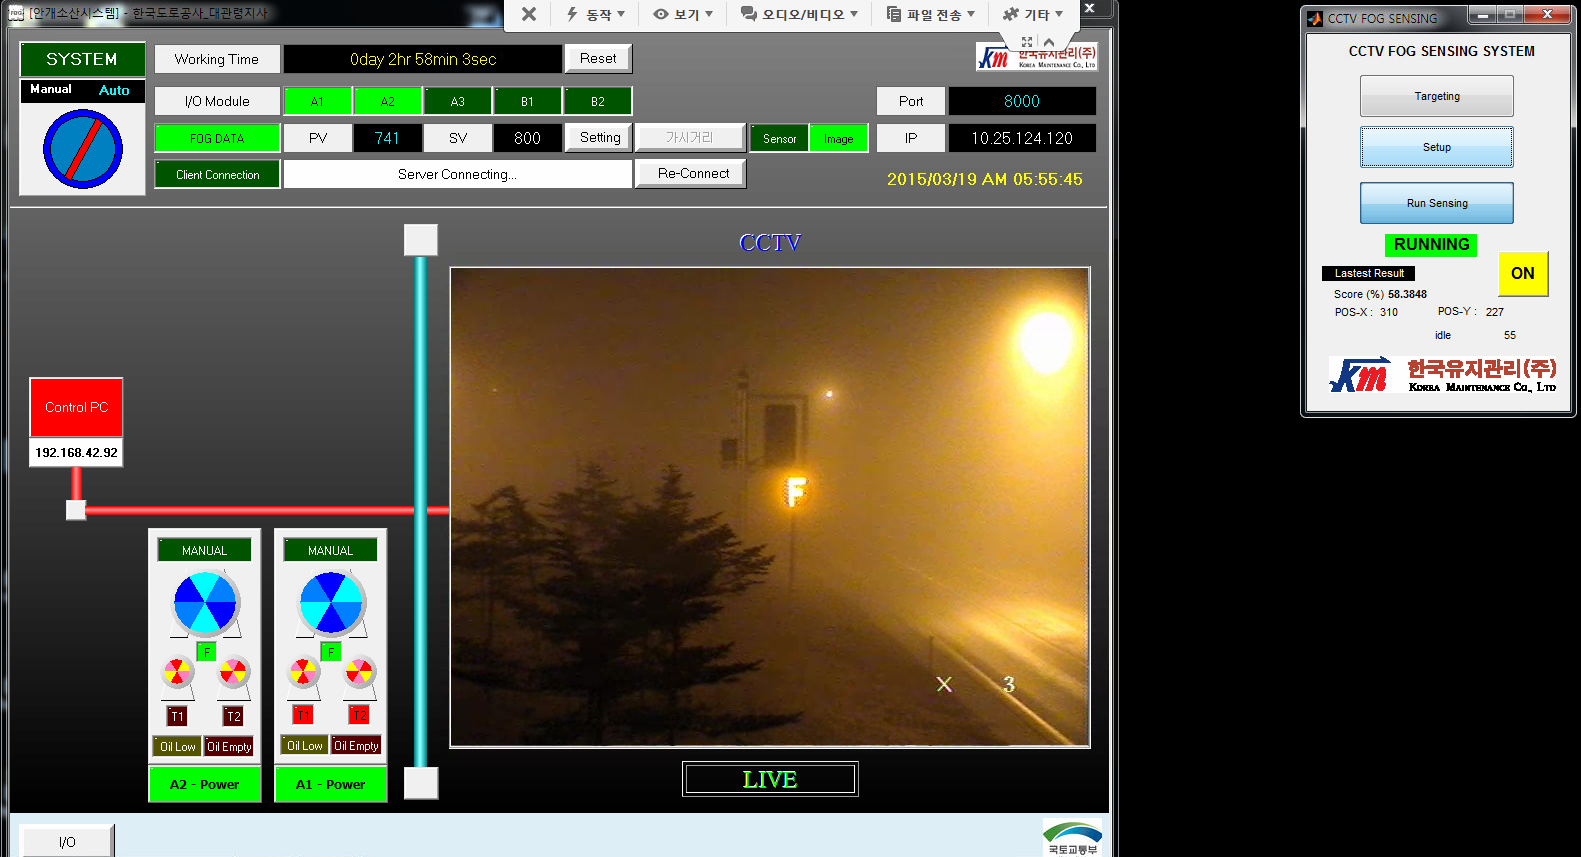
\includegraphics[width=1.2\textwidth]{images/fog_02_01.png}
				      \caption*{Fog cannon controller}
			      }\qquad
			      \parbox{0.3\textwidth}{
				      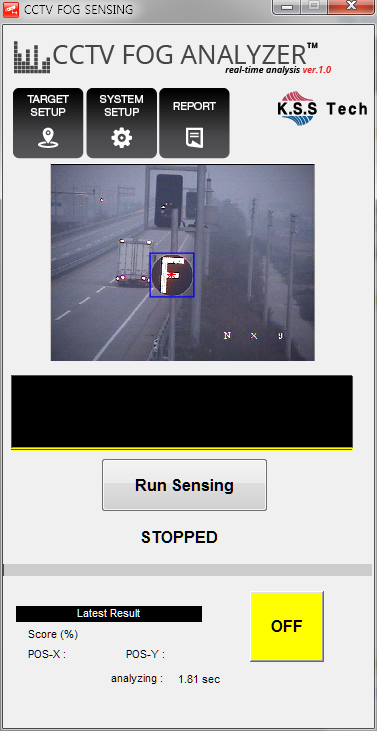
\includegraphics[width=0.3\textwidth]{images/fog_03.png}
				      \caption*{시정거리 계산 / PID 제어}
			      }
		      \end{fullwidth}
	      \end{figure}
\end{itemize}

\divider

\cvevent{\printinfo{\faPlusSquare}{능동형 제진장치 (\href{http://www.sciencedirect.com/science/article/pii/S0141029697000722}{Active \& Hybrid Mass Damper, A-HMD})개발 및 웹플랫폼 개발}}{Korea Maintenance \& APROS 개발참여: 100\%}{2014 -- 2019}{Seoul, Korea}

\begin{itemize}
	\item 소개: 건물의 사용중 진동 저감을 위한 능동형 제진장치 설치 및 모니터링 플랫폼 개발 프로젝트
	\item 참여 개발 내용:
	      \begin{itemize}
		      \item \href{http://www.quanser.com/products/active_mass_damper}{Quansar 소형 AMD 제어}, \href{https://en.wikipedia.org/wiki/Linear-quadratic_regulator}{LQR}/\href{https://en.wikipedia.org/wiki/Linear-quadratic-Gaussian_control}{LQG} 알고리즘 탑재.
		      \item 실제 현장에서 계측데이터 품질 확보를 위한 signal conditioning
		      \item High-resolution DAQ 적용
		      \item Raspberry Pi를 이용한 PLC, DAQ, Anemometer 데이터 송출
		      \item MQTT Broker를 통한 데이터 표출 API 개발
		      \item 모니터링 웹애플리케이션 개발
	      \end{itemize}
	      \begin{figure}[!ht]
		      \begin{fullwidth}
			      \parbox{0.5\textwidth}{
				      \centering
				      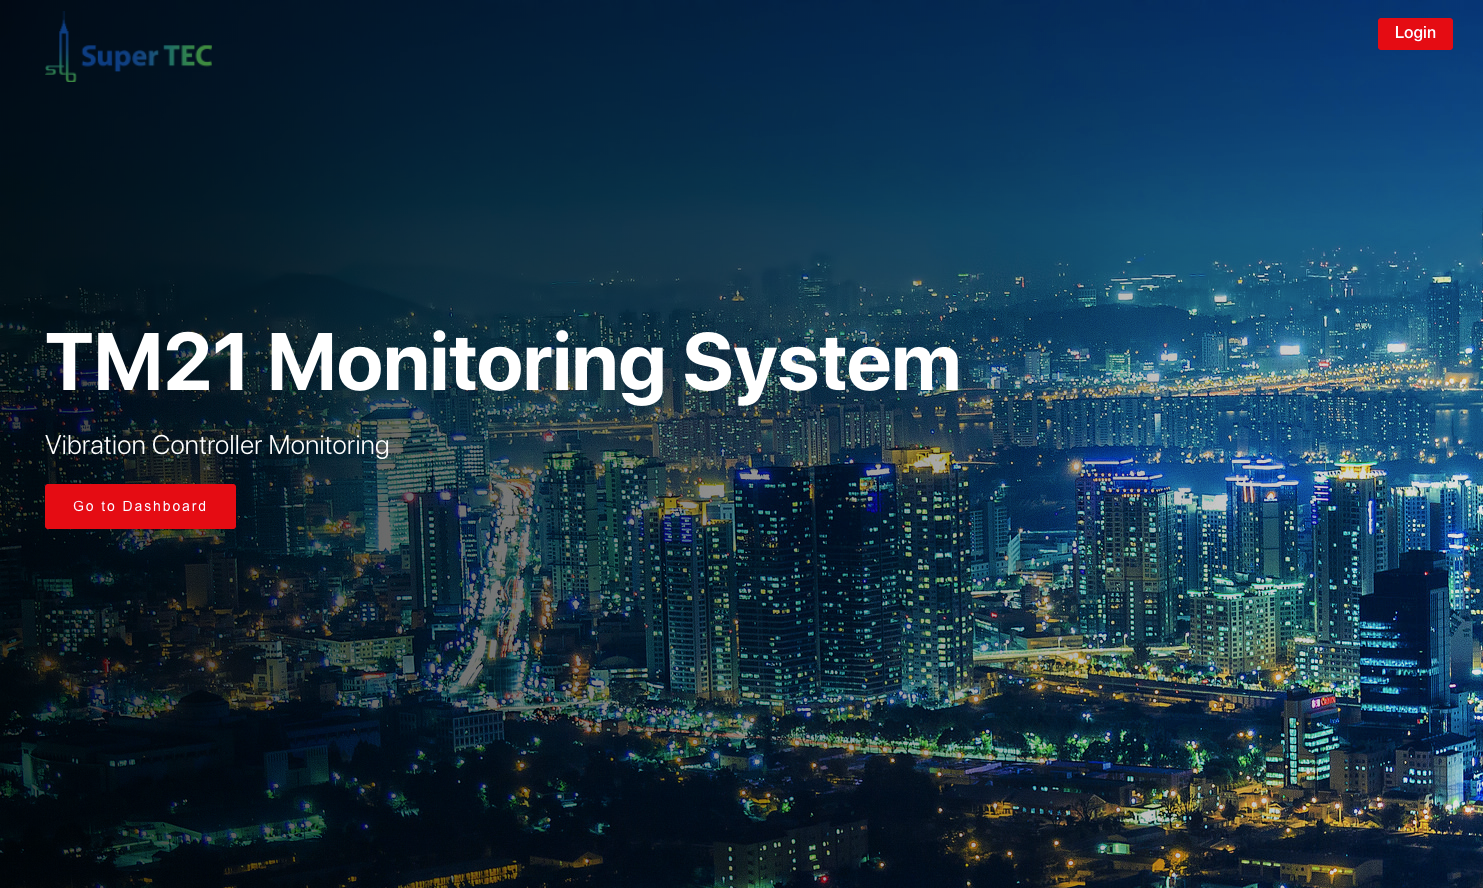
\includegraphics[width=0.5\textwidth]{images/TM21 Vibration Controller Monitroing - landing.png}
				      \caption*{Landing page}
			      }\qquad
			      \parbox{0.5\textwidth}{
				      \centering
				      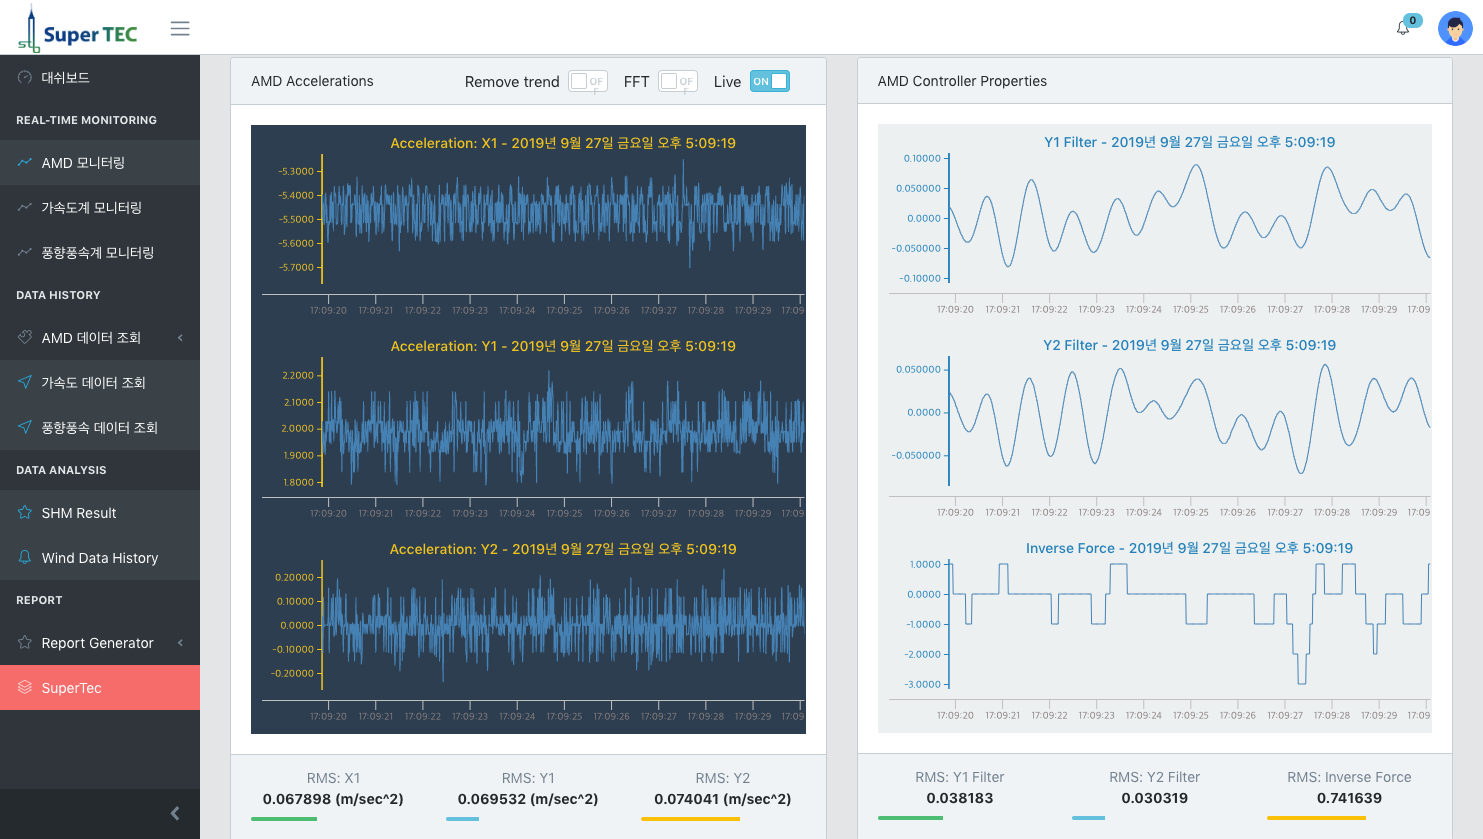
\includegraphics[width=0.5\textwidth]{images/TM21 Vibration Controller Monitroing - amd1}
				      \caption*{RT AMD mon \#1}
			      }\qquad
			      \parbox{0.5\textwidth}{
				      \centering
				      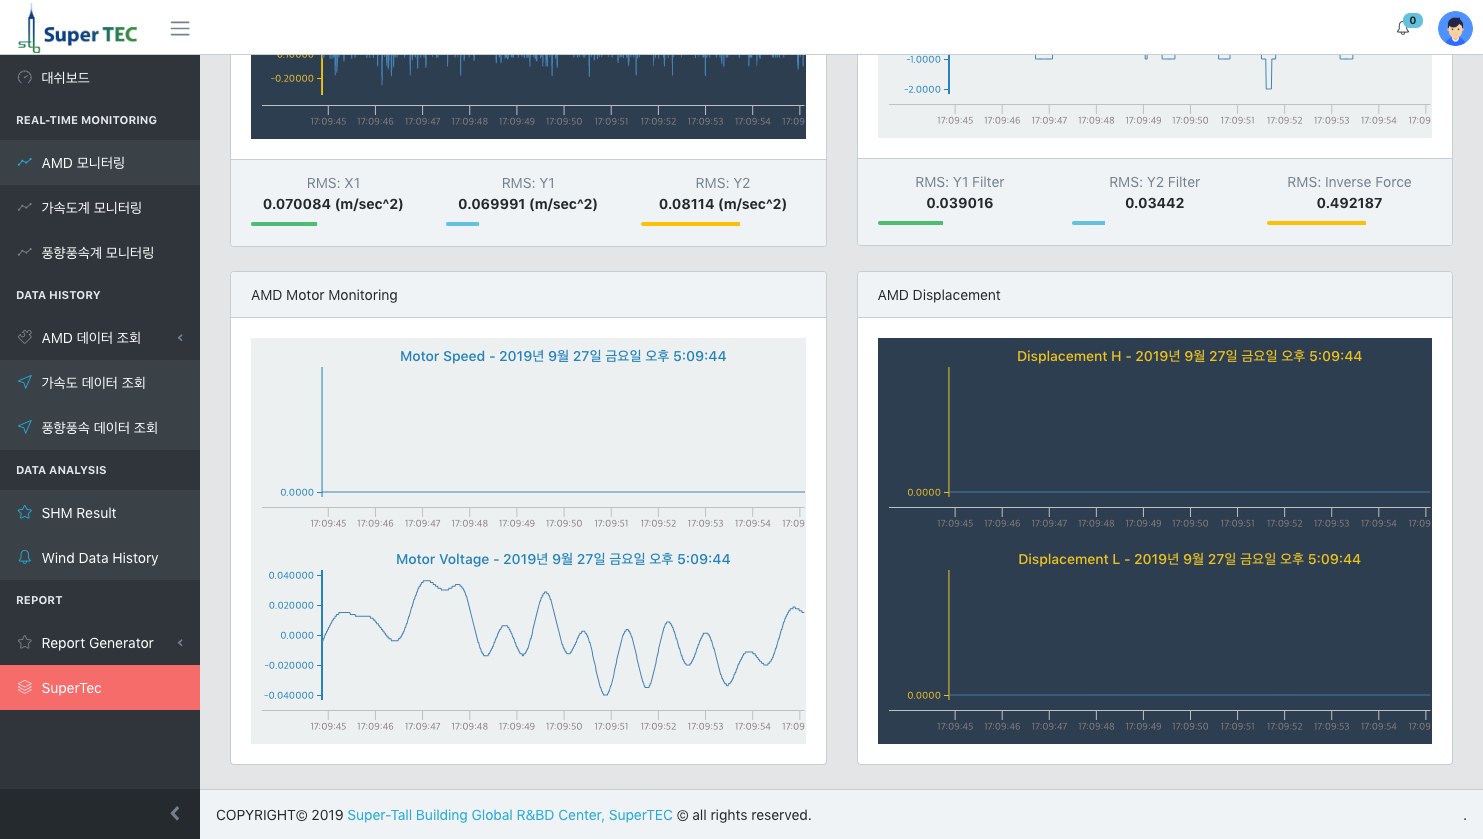
\includegraphics[width=0.5\textwidth]{images/TM21 Vibration Controller Monitroing - amd2}
				      \caption*{RT AMD mon \#2}
			      }
			      \parbox{0.5\textwidth}{
				      \centering
				      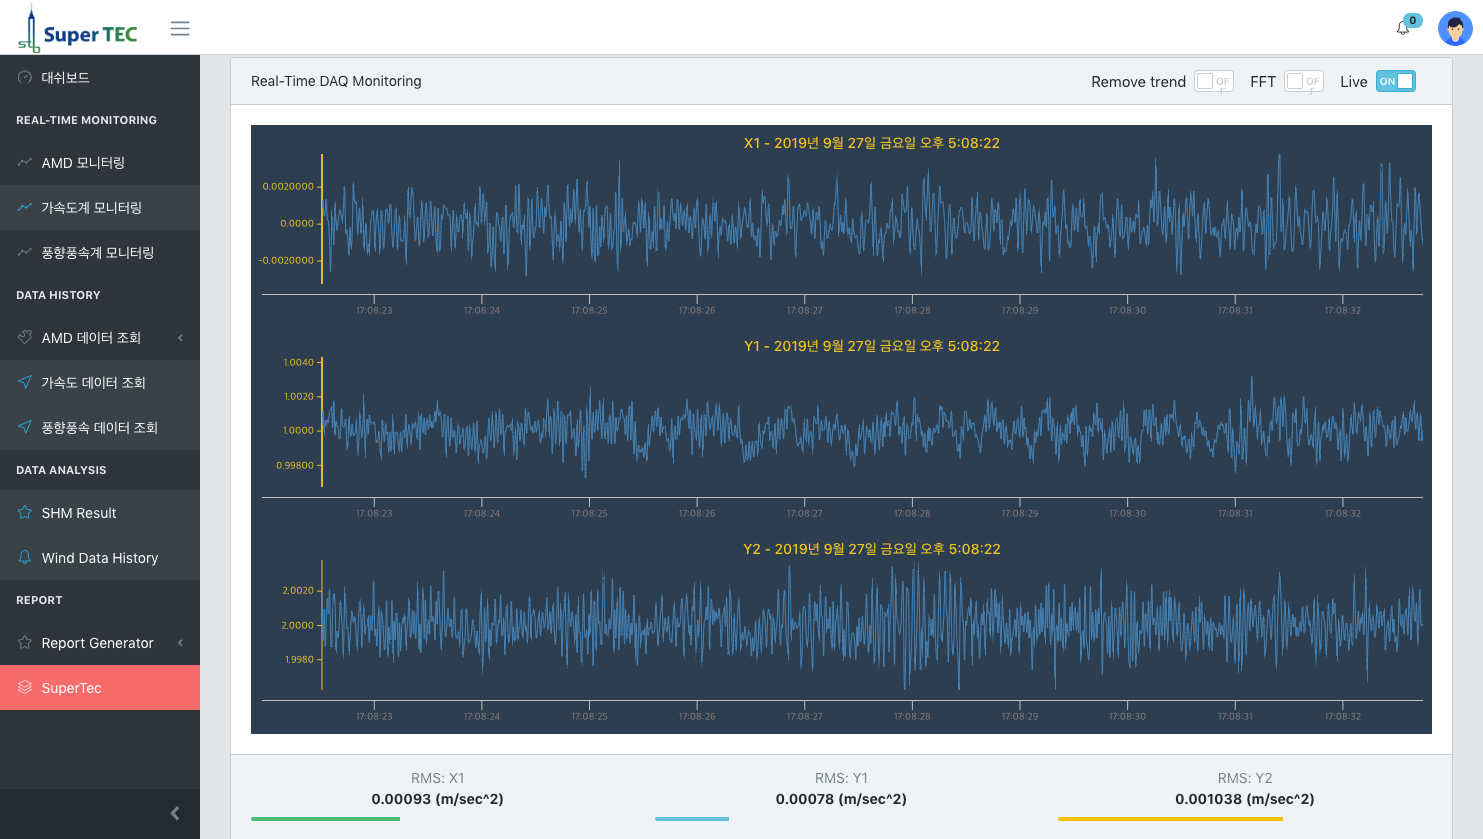
\includegraphics[width=0.5\textwidth]{images/TM21 Vibration Controller Monitroing - time2}
				      \caption*{RT Acc. mon. Time domain}
			      }\qquad
			      \parbox{0.5\textwidth}{
				      \centering
				      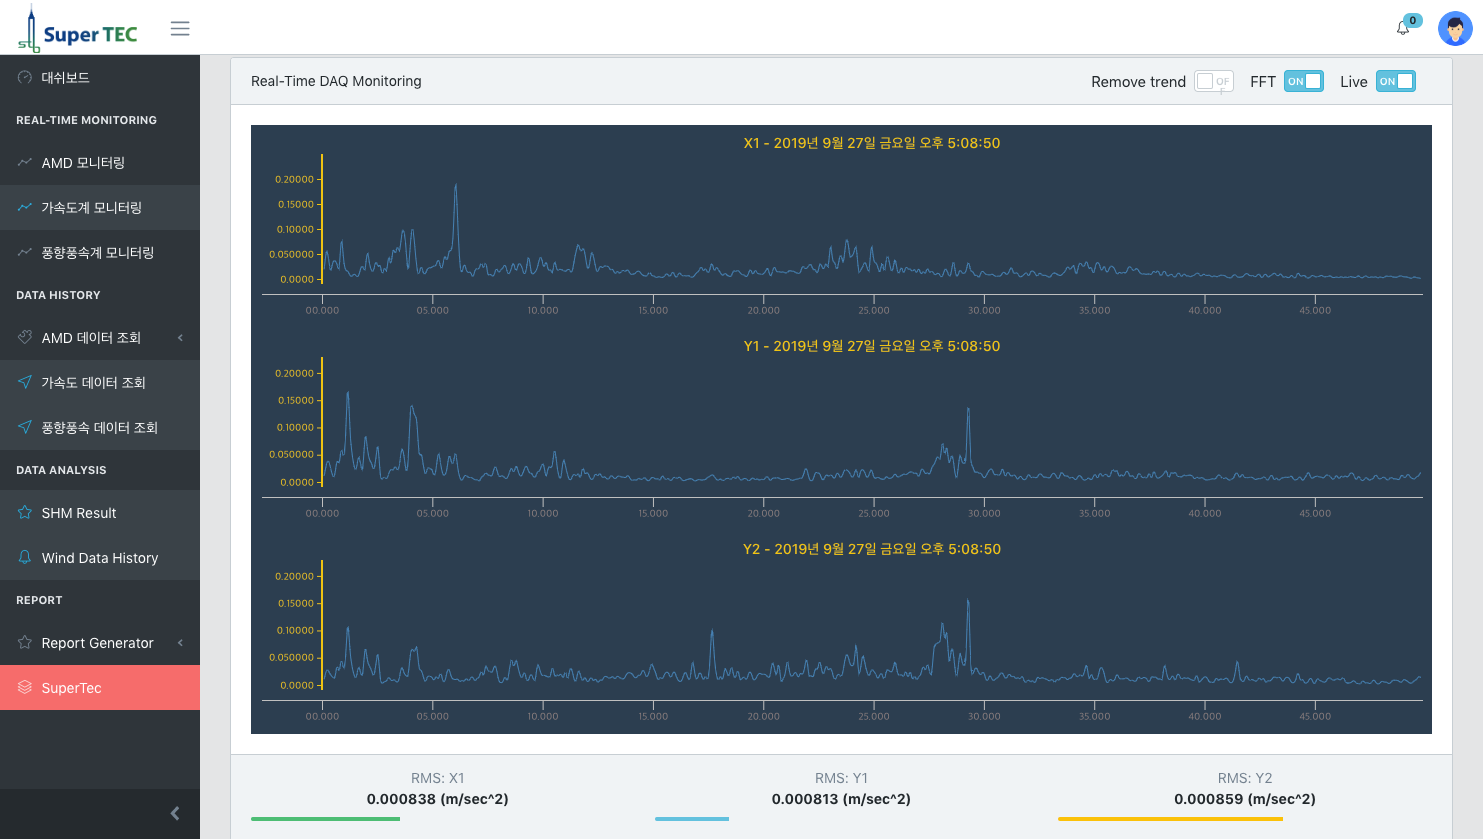
\includegraphics[width=0.5\textwidth]{images/TM21 Vibration Controller Monitroing - fft2}
				      \caption*{RT Acc. mon. Frequency domain}
			      }\qquad
			      \parbox{0.5\textwidth}{
				      \centering
				      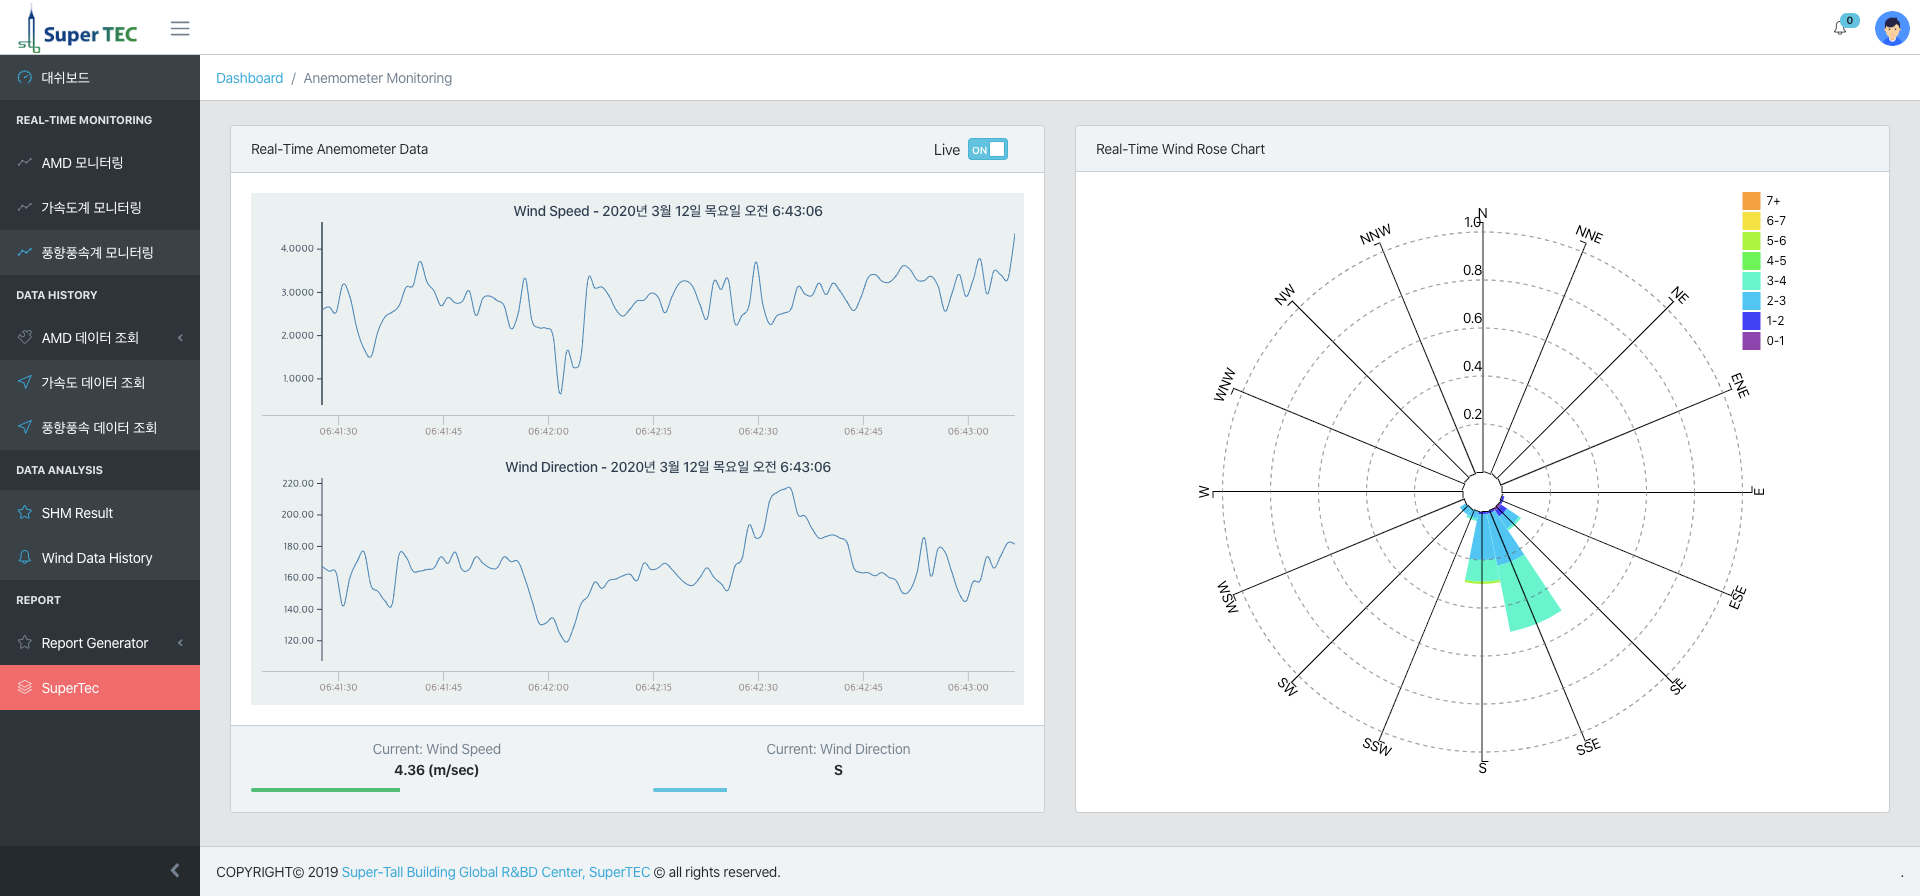
\includegraphics[width=0.5\textwidth]{images/TM21 Vibration Controller Monitroing - 220.149.227.106}
				      \caption*{RT. Wind mon.}
			      }
		      \end{fullwidth}
	      \end{figure}
	\item
	      적용된 기술:
	      \begin{itemize}
		      \item \href{https://en.wikipedia.org/wiki/Linear-quadratic_regulator}{LQR}/\href{https://en.wikipedia.org/wiki/Linear-quadratic-Gaussian_control}{LQG} control algorithm
		      \item \href{https://en.wikipedia.org/wiki/Sliding_mode_control}{sliding mode control}\footnote{In control system,  \href{https://en.wikipedia.org/wiki/Sliding_mode_control}{sliding mode control, or SMC}, is a nonlinear control method that alters the dynamics of a nonlinear system by application of a discontinuous control signal that forces the system to ``slide'' along a cross-section of the system's normal behavior.} algorithm
		      \item \href{https://en.wikipedia.org/wiki/Minor_loop_feedback}{velocity feedback control} algorithm
		      \item \href{http://www.ti.com/lit/ds/symlink/ads1282-ht.pdf}{ADS1282-HT (High-Resolution Analog-To-Digital Conversion)}
		      \item Signal conditioning
		      \item \href{https://en.wikipedia.org/wiki/Programmable_logic_controller}{PLC(Programmable Logic Controller)}
		      \item Javascript(ES5), NodeJS, Express, GraphQL
		      \item Socket.io
		      \item MQTT (CBOR)
		      \item MongoDB
		      \item ReactJS
	      \end{itemize}
	\item 개발 스택 및 프레임워크
	      \begin{itemize}
		      \item Mathworks MATLAB / GUI / Simulink
		      \item National Instruments LabVIEW
		      \item nodeJS
	      \end{itemize}
	\item 참여한 현장: 강변 테크노마트 AMD 시공 프로젝트
\end{itemize}


\divider

\cvevent{\printinfo{\faPlusSquare}{초고층건물 구조건전도 모니터링}\href{https://en.wikipedia.org/wiki/Structural_health_monitoring}{Structural Health Monitoring}\footnote{The process of implementing a damage detection and characterization strategy for engineering structures is referred to as \href{https://en.wikipedia.org/wiki/Structural_health_monitoring}{Structural Health Monitoring (SHM)}}}{Korea Maintenance CO., LTD. 개발참여: 97\%}{2011 -- 2012}{Seoul, Korea}

\begin{itemize}
	\item 소개: 초고층건물의 시공중/사용중 계측 모니터링 : 주로 FBG, 지진가속도계, 가속도계, GPS, 풍향풍속계 사용.
	\item 참여 개발 내용
	      \begin{itemize}
		      \item \href{https://en.wikipedia.org/wiki/Signal-to-noise_ratio}{SNR} 125dB\textasciitilde{}130dB 이상의 센서에 적합한 \href{https://en.wikipedia.org/wiki/Data_acquisition}{DAQ} 보드 개발: 저주파와 신호대잡음비 성능이 우수한 가속도계 센서에 적합한 \href{https://en.wikipedia.org/wiki/Data_acquisition}{DAQ}는 사실상 고가임. 따라서 설치가 용이한 유선 네트워크방식의 \href{https://en.wikipedia.org/wiki/Data_acquisition}{DAQ}보드 개발이 필요하여 개발참여.
		      \item \href{http://kr.mathworks.com/help/daq/examples/getting-started-with-session-based-interface-using-ni-devices.html}{Session-based interface} 프로그래밍으로 데이터수집을 다른 thread로 작동시킴과 동시에 분석과 해석이 동시에 이루어짐 (실시간 모드벡터 추출/FFT또는 파워스펙트럼 그래프도시)
		            \begin{figure}[ht]
			            \begin{fullwidth}
				            \parbox{0.5\textwidth}{
					            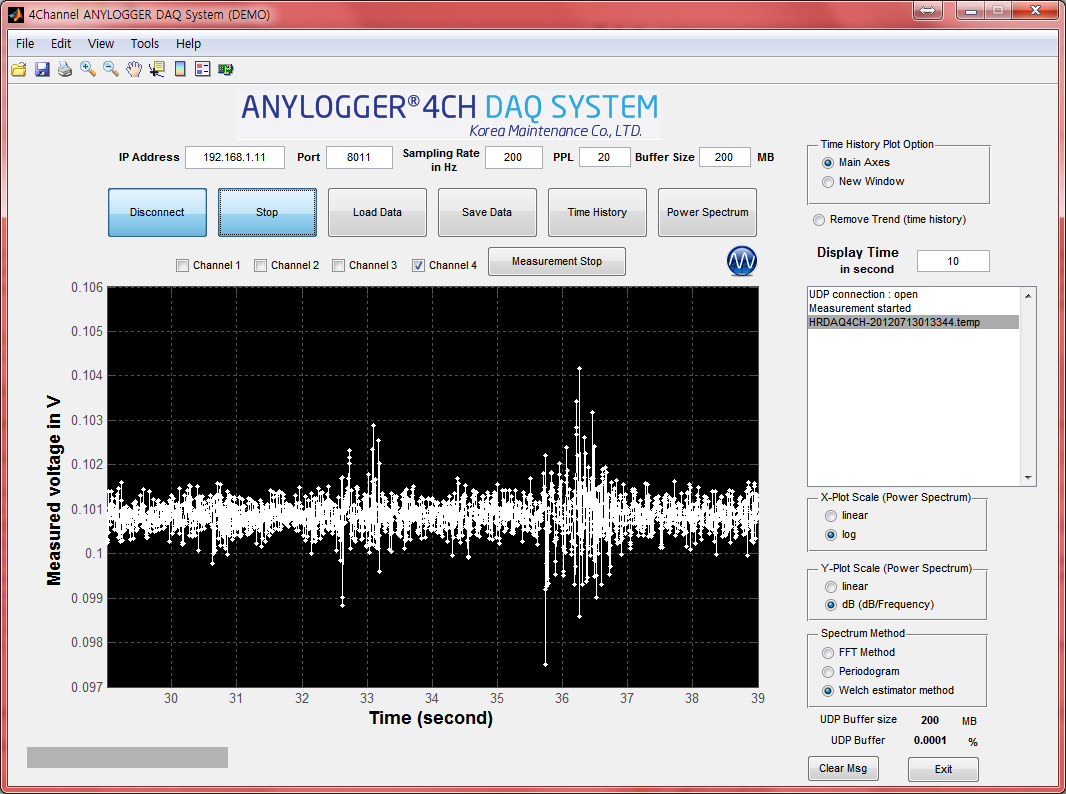
\includegraphics[width=0.5\textwidth] {images/SW1.JPG}
					            \caption*{Time series}
				            }\qquad
				            \parbox{0.5\textwidth}{
					            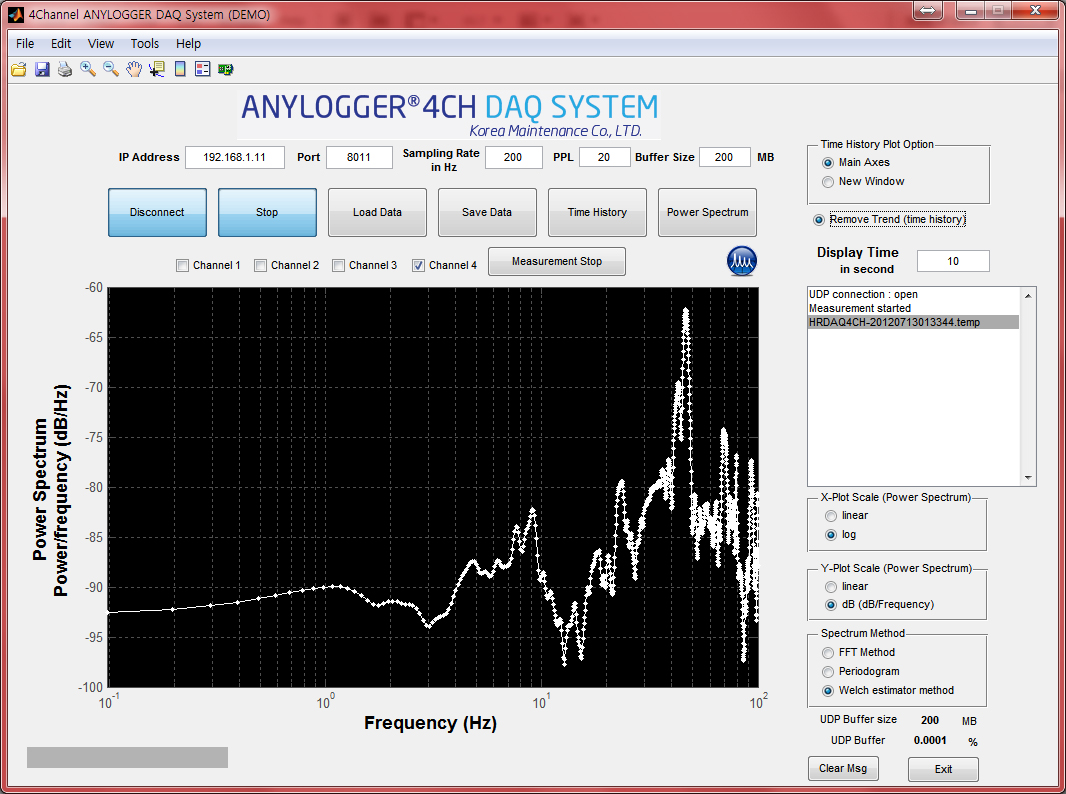
\includegraphics[width=0.5\textwidth] {images/SW2.JPG}
					            \caption*{Frequency domain}
				            }\qquad
				            \parbox{0.5\textwidth}{
					            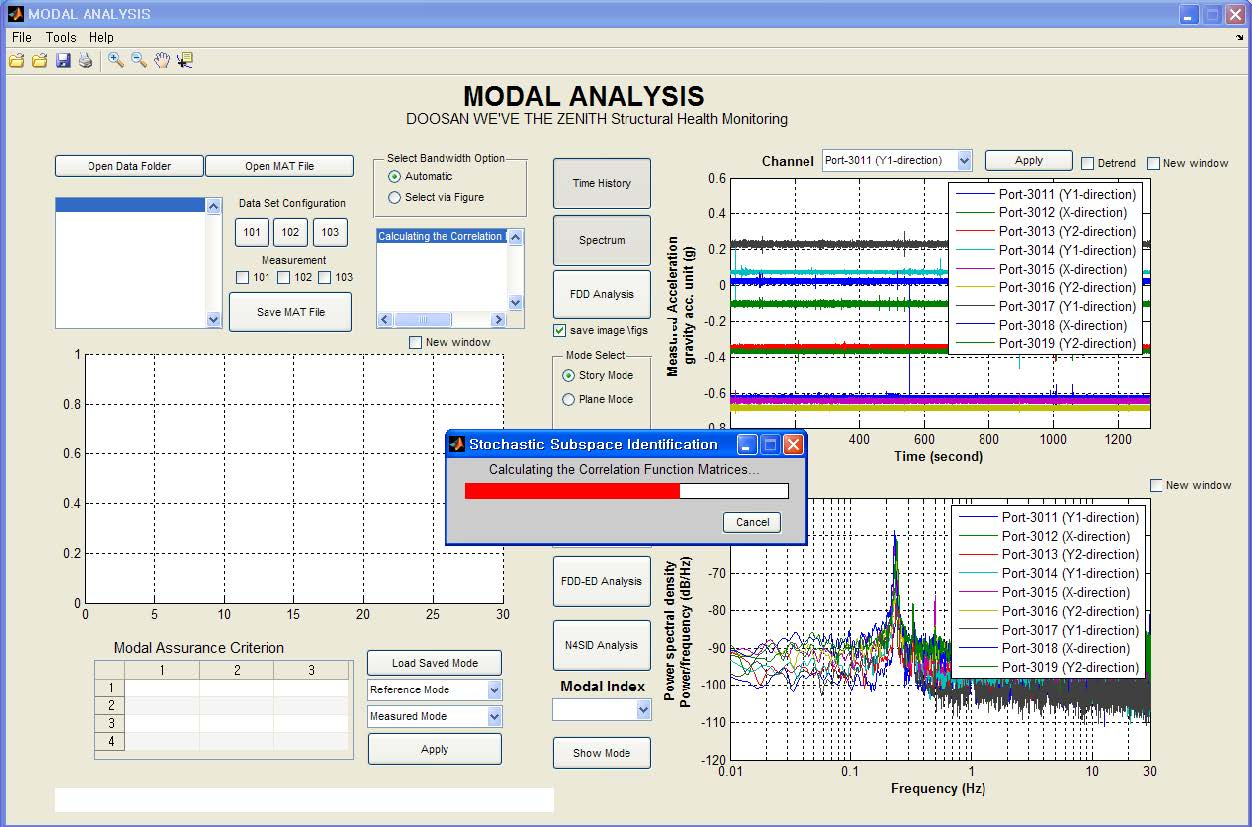
\includegraphics[width=0.5\textwidth] {images/doosan_01.jpg}
					            \caption*{Modal analysis (FDD/SSI)}
				            }
			            \end{fullwidth}
		            \end{figure}
		      \item 시각동기화 프로토콜 적용 \href{https://ko.wikipedia.org/wiki/IEEE_1588}{IEEE-1588 Precision Time Protocol}\footnote{Precision Time Protocol(PTP)은 네트워크 간 정확한 동기화를 가능케하는 \href{https://ko.wikipedia.org/wiki/IEEE_1588}{IEEE 1588} 표준 시간 전송 프로토콜이다. 하드웨어에서 생성하는 타임스탬프를 사용할 때 나노초 단위의 정확도까지 보장해 준다.} : GPS 클럭을 모든 장비에 연결하려면 많은 인력과 비용이 소모됨. 따라서 유선네트워크 방식에서의 동기화 프로토콜을 적용 (펌웨어단계에서 클럭동기화에 성공)
		      \item 지진경보 시스템 : 여러동의 건물의 경우 각동 지하에 지진가속도계를 설치하여 지진경보를 발령. 이때 각동의 EPGA\footnote{In seismic engineering, the effective peak acceleration (EPA, the maximum ground acceleration to which a building responds) is often used, which tends to be ⅔ -- ¾ the PGA, The term `\href{http://www.teachmefinance.com/Scientific_Terms/Effective\%20peak\%20ground\%20acceleration.html\#ixzz3iNuQcQLs}{Effective peak ground acceleration}' as it applies to the area of reclamation can be defined as `That acceleration which is most closely related to structural response and to damage potential of an earthquake'.}값으로 rms-triggering 적용 각 3개의 동에서 동시에 임계값 이상이 발생하였을 때 지진으로 판정.
		      \item 모드정보 추출 : SSI(Stochastic subspace identification)\footnote{The data driven \href{http://www.svibs.com/solutions/literature/2006_2.pdf}{\textbf{Stochastic Subspace Identification}} techniques is considered to be the most powerful class of the known identification techniques for natural input modal analysis in the time domain. Refer to B. Peeters and G. D. Rodeck (1999), ``\href{ftp://193.136.28.78/pub/Personal/Dec/filipema/public/FCT_WindOMA/ref_8.pdf}{Reference-based Stochastic Subspace Identification for Output-only Modal Analysis}'', \emph{Mechanical Systems and Signal Processing} (1999) 13(6), 855\}878} 기법과 \href{https://en.wikipedia.org/wiki/Frequency_domain_decomposition}{FDD(Frequency domain decomposition)}\footnote{The \href{https://en.wikipedia.org/wiki/Frequency_domain_decomposition}{frequency domain decomposition (FDD)} is an output-only system identification technique popular in civil engineering, in particular in structural health monitoring. As an output-only algorithm, it is useful when the input data is unknown. FDD is a modal analysis technique which generates a system realization using the frequency response given (multi-)output data} 기법을 적용
	      \end{itemize}
	      \begin{figure}[ht]
		      \begin{fullwidth}
			      \parbox{0.8\textwidth}{
				      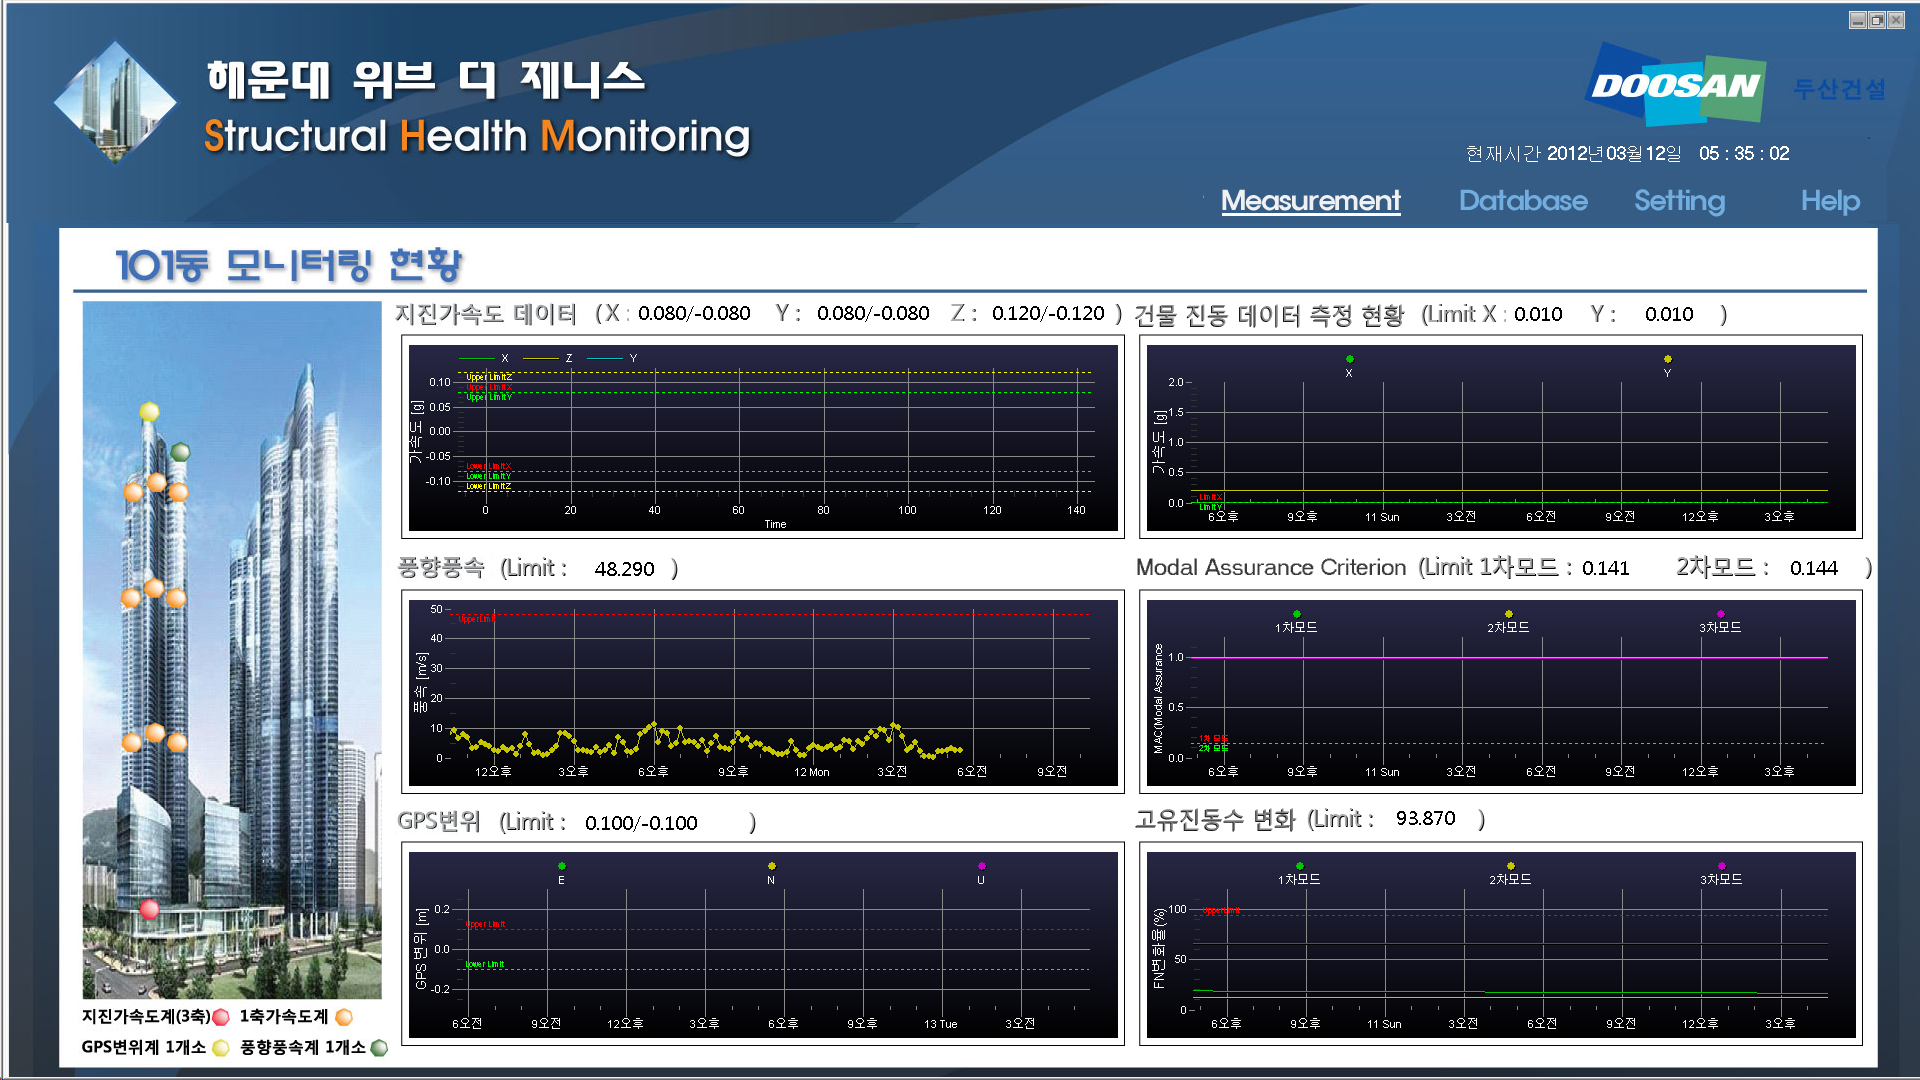
\includegraphics[width=0.8\textwidth] {images/M3.PNG}
				      \caption*{Main}
			      }\qquad
			      \parbox{0.8\textwidth}{
				      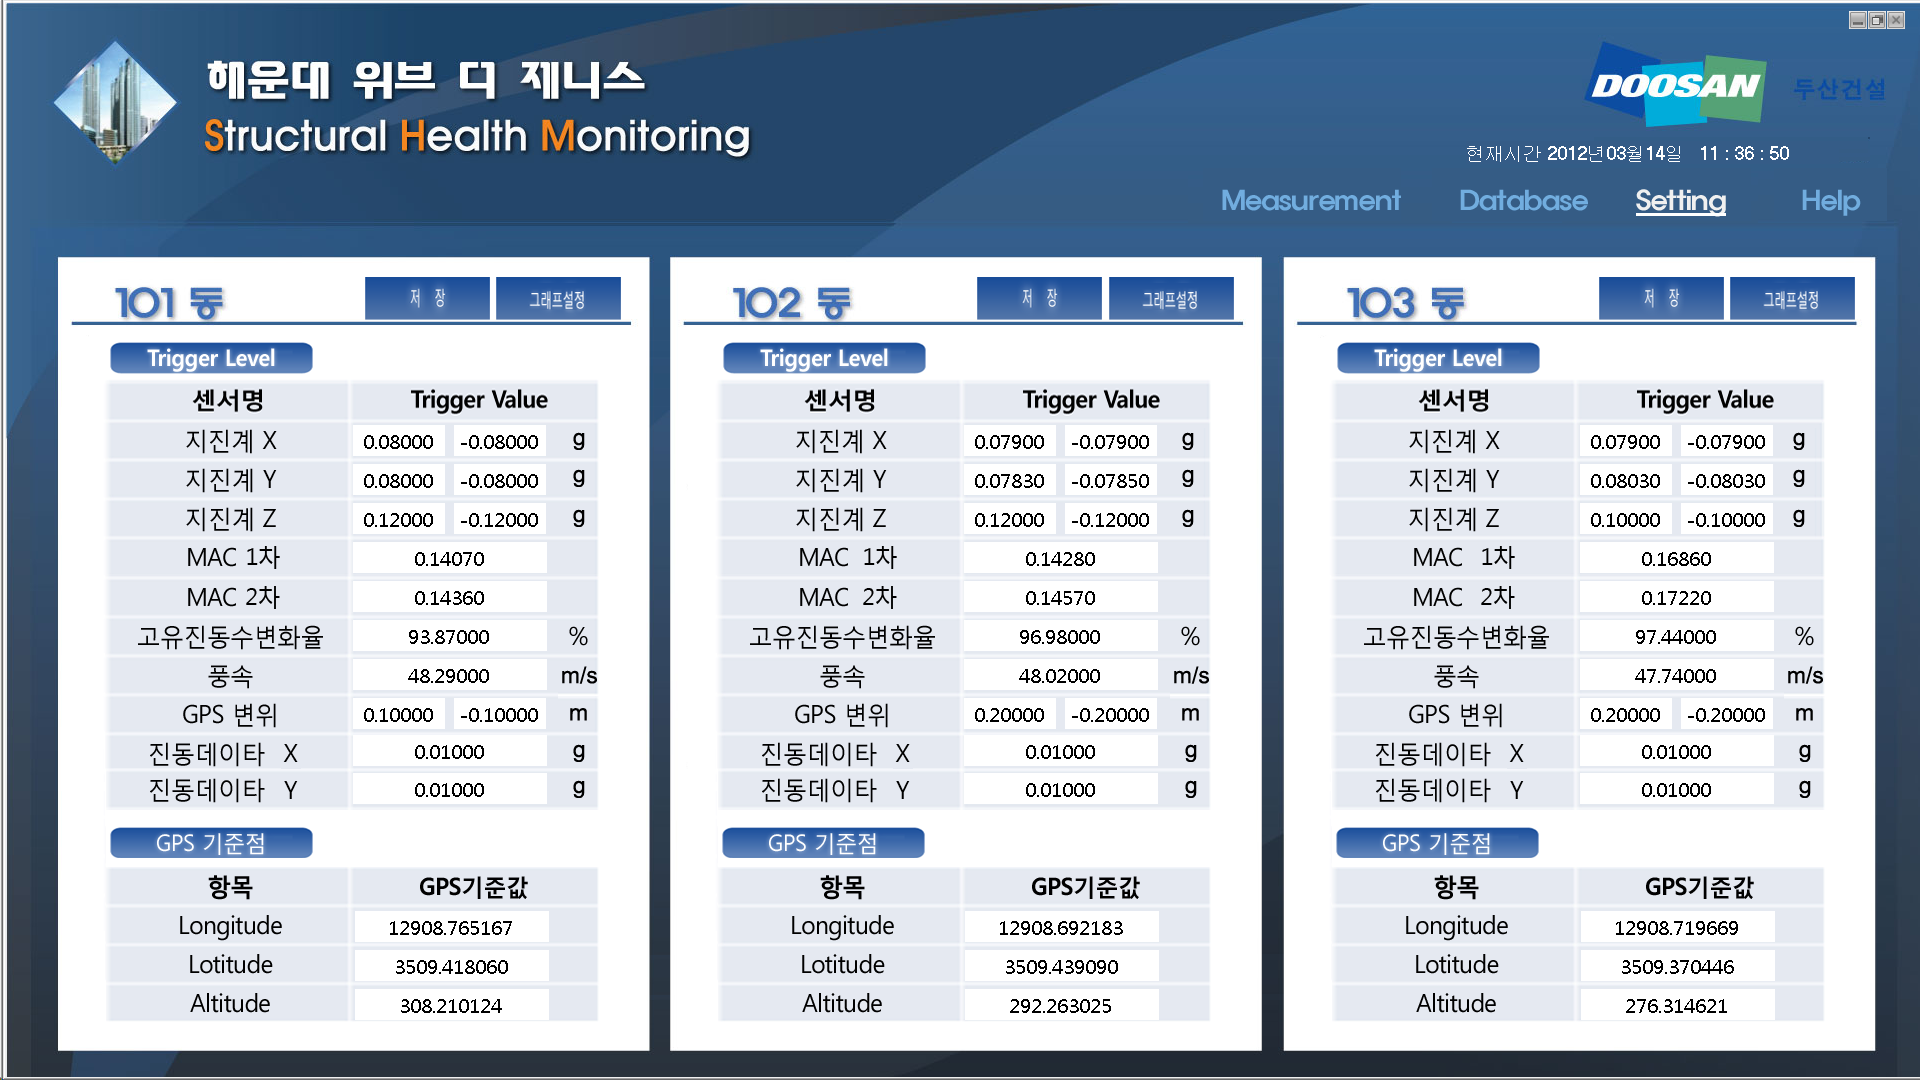
\includegraphics[width=0.8\textwidth] {images/M9.PNG}
				      \caption*{Details}
			      }
		      \end{fullwidth}
	      \end{figure}
	\item 적용된 기술:
	      \begin{itemize}
		      \item \href{http://kr.mathworks.com/products/daq/}{Data acquisition toolbox (MATLAB)}
		      \item \href{https://ko.wikipedia.org/wiki/IEEE_1588}{IEEE-1588 Precision Time Protocol}
		      \item High-Resolution Analog-To-Digital Conversion
		      \item Stochastic subspace identification
		      \item Frequency domain decomposition
		      \item \href{https://en.wikipedia.org/wiki/Eigensystem_realization_algorithm}{Eigensystem Realization Algorithm}
		      \item \href{https://en.wikipedia.org/wiki/Finite_element_updating}{FE Model update}\footnote{\href{https://en.wikipedia.org/wiki/Finite_element_updating}{Finite element model updating} is the process of ensuring that finite element analysis results in models that better reflect the measured data than the initial models. It is part of verification and validation of numerical models.} / \href{https://en.wikipedia.org/wiki/System_identification}{System Identification}\footnote{The field of \href{https://en.wikipedia.org/wiki/System_identification}{system identification} uses statistical methods to build mathematical models of dynamical systems from measured data. System identification also includes the optimal design of experiments for efficiently generating informative data for fitting such models as well as model reduction.}
	      \end{itemize}
	\item 개발 스택 및 프레임워크: Mathworks MATLAB / GUI
	\item 참여한 현장:
	      \begin{itemize}
		      \item 부산 해운대 두산위브더제니스 (사용중계측 SHM)
		      \item 인천 송도 NEATT 동북아무역센터 (시공중계측)
		      \item 롯데 잠실 슈퍼타워 (RFP지원\&자문)
		      \item 송도 M1 주상복합 (자문)
	      \end{itemize}
\end{itemize}

\divider

\cvevent{\printinfo{\faPlusSquare}{LCD Display 글래스 이송로봇진동 사전감지시스템 (\href{https://en.wikipedia.org/wiki/Early_warning_system}{Early Warning System})}}{Korea Maintenance CO., LTD. 개발참여: 90\%}{2011 -- 2012}{Seoul, Korea}

\begin{itemize}
	\item 소개: Glass를 옮기는 이송로봇에 3축가속도계 1기 설치하여 로봇관절운동의 패턴을 분류하고 초기치에 비해 변화량을 모니터링 해서 각 파트의 이상을 미리 감지.
	\item 프로젝트 목표: 제조사측은 사전진단(\href{https://en.wikipedia.org/wiki/Early_warning_system}{Eearly Warning System, EWS})과 부품별 파트진단(\href{https://en.wikipedia.org/wiki/Predictive_maintenance}{Prediction Management Program, PMP})을 수행하기 원함.
	\item 참여 개발 내용
	      \begin{itemize}
		      \item 신호분리기법 적용: \href{https://en.wikipedia.org/wiki/Hankel_matrix}{Hankel Matrix}와 \href{https://en.wikipedia.org/wiki/Singular_value_decomposition}{Singular value decomposition, SVD}기법을 활용해서 signal decomposition 적용 그리고 \href{https://en.wikipedia.org/wiki/Wavelet}{wavelet} 기법을 적용해서 신호분리도 적용 \item 패턴분류: rms-triggering기법으로 구간을 나눈후 \href{https://en.wikipedia.org/wiki/Independent_component_analysis}{ICA(independent component analysis)}적용
		      \item Spectrogram과 Cepstrum 분석으로 사전진단 가능성 판단
		      \item 각관절의 기어박스, rotor의 엔코더 데이터를 받아서 order-analysis 를 수행하여야 정확한 파트이상진단까지 할 수 있었으나 비용등의 문제로 더이상 진행하지 못함.
		      \item 중소기업 과제로 변경 수행완료
	      \end{itemize}
	\item 적용된 기술:
	      \begin{itemize}
		      \item Hankel matrix based signal decomposition\footnote{The linear sum of a series of component signals by Hankel matrix-based SVD, and essentially what the component signals reflect are projections of original signal on the orthonormal bases of m-dimensional and n-dimensional vector spaces. Refer to Xuezhi Zhao, , Bangyan Ye(2009),  ``\href{http://www.sciencedirect.com/science/article/pii/S0888327008002604}{Similarity of signal processing effect between Hankel matrix-based SVD and wavelet transform and its mechanism analysis}'', \emph{Mechanical Systems and Signal Processing} Volume 23, Issue 4, May 2009, Pages 1062--1075}
		      \item Wavelet analysis
		      \item \href{https://en.wikipedia.org/wiki/Independent_component_analysis}{Independent component analysis}
		      \item \href{https://en.wikipedia.org/wiki/Cepstrum}{Cepstrum analysis}\footnote{A cepstrum is the result of taking the Inverse Fourier transform (IFT) of the logarithm of the estimated spectrum of a signal.}
		      \item \href{https://en.wikipedia.org/wiki/Spectrogram}{Spectrogram}
	      \end{itemize}
	      \begin{figure}[ht]
		      \begin{fullwidth}
			      \parbox{0.8\textwidth}{
				      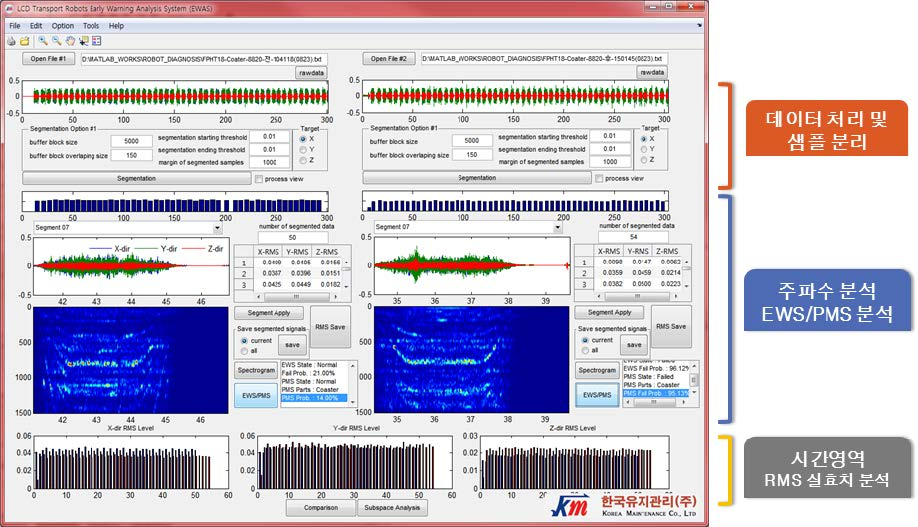
\includegraphics[width=0.8\textwidth]{images/lgdisplay.jpg}
				      \caption*{Time series}
			      }\qquad
			      \parbox{0.8\textwidth}{
				      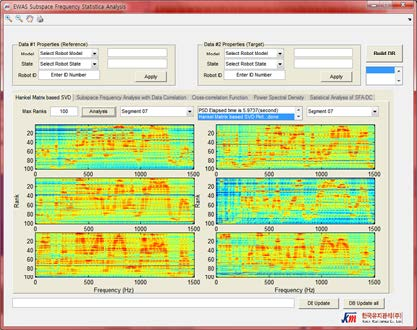
\includegraphics[width=0.8\textwidth]{images/lgdisplay_02.jpg}
				      \caption*{Frequency domain}
			      }
		      \end{fullwidth}
	      \end{figure}
	\item 개발 스택 및 프레임워크: Mathworks MATLAB / GUI
	\item 참여한 현장: LG Display 파주공장
\end{itemize}

\divider

\cvevent{\printinfo{\faPlusSquare}{코레일 공항철도 및 KTX 진동가속도 분석 시스템}}{Korea Maintenance CO., LTD. 개발참여: 95\%}{Oct. 2011 -- Sep. 2012}{Seoul, Korea}

\begin{figure}[ht]
	\begin{fullwidth}
		\centering
		\parbox{0.5\textwidth}{
			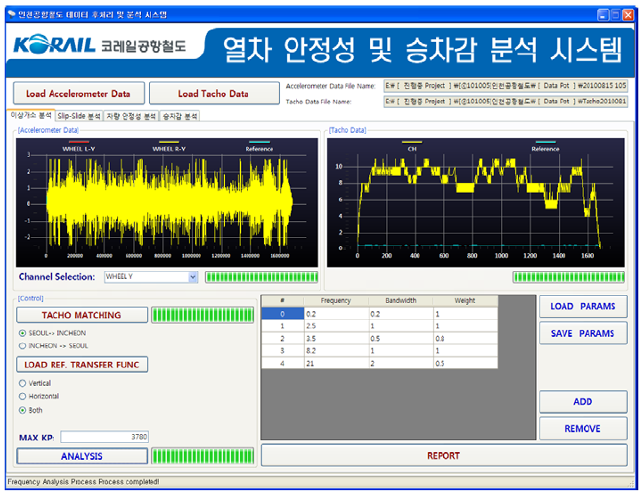
\includegraphics[width=0.5\textwidth] {images/arex_01.png}
			\caption*{궤도 이상개소 분석}
		}\qquad
		\parbox{0.5\textwidth}{
			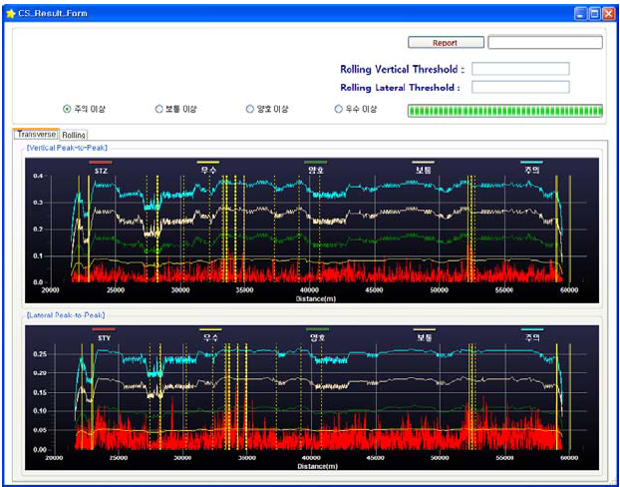
\includegraphics[width=0.5\textwidth] {images/arex_02.png}
			\caption*{주행 안정성 분석}
		}\qquad
		\parbox{0.5\textwidth}{
			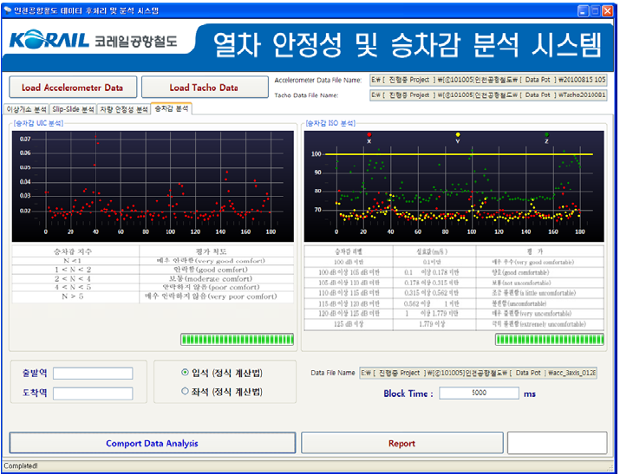
\includegraphics[width=0.5\textwidth] {images/arex_03.png}
			\caption*{열차 승차감 분석}
		}
	\end{fullwidth}
\end{figure}

\begin{itemize}
	\item 소개 : 차축-대차-차체의 좌우 2방향 가속도계 설치, 차축의 타코미터 설치, 계측시스템을 구성하여 공항철도의 궤도이상개소검출, 열차의 주행안정성평가, \href{http://ieeexplore.ieee.org/xpl/login.jsp?tp=\&arnumber=264942\&url=http\%3A\%2F\%2Fieeexplore.ieee.org\%2Fxpls\%2Fabs_all.jsp\%3Farnumber\%3D264942}{slip/slide} 및 승차감평가 시스템 개발 및 준공
	\item 참여 개발 내용:
	      \begin{itemize}
		      \item 공항철도 이상개소 분석시스템 : 10m KP간격 CWA-FRF\footnote{Coherence Weighted Averaged Frequency Response Function (CWA-FRF) refer to ``\href{http://institute.lanl.gov/ei/shm/pubs/modal_stat_jvc_jul00.pdf}{Estimation Of Statistical Distributions For Modal Parameters Identified From Averaged Frequency Response Function Data}'', Journal of Vibration and Control, July 2000} 함수로 전달함수 예측, 측정된 차축-대차-차체의 \href{https://en.wikipedia.org/wiki/Frequency_response}{주파수응답함수(Frequency response function, FRF)}를 통해 중심주파수-대역폭-가중치함수를 규정, \href{http://www.scholarpedia.org/article/Boundary_value_problem}{경계비선형} 최적화 알고리즘 적용으로 이상개소 분석시스템 구축
		      \item 공항철도 차량 주행 안정성 분석 시스템 : 병진, 롤링진동 분석 후 속도/도상 별 기준값 적용하여 이상진동의 위치 검출
		      \item 공항철도/도시철도 승차감 분석 시스템 : \href{http://www.iso.org/iso/catalogue_detail.htm?csnumber=7612}{ISO 2631-1:1997}과 \href{http://www.uic.org/etf/codex/codex-detail.php?codeFiche=513\&langue_fiche=E}{UIC513}에서 제시한 방법으로 각각 필터제작 4채널 DAQ보드와 3축 가속도계 센서 적용
		      \item 공항철도 slip/slide : 타코미터의 펄스의 계측노이즈 정규화 제거하고 속도 수치미분으로 임계값으로 정성적으로 판단. 실제 주행거리와 slip/slide 개소와 그 거리는 대부분 일치함으로 확인.
		      \item KTX 주행거동평가 알고리즘 : 국내에서 개발한 KTX산천, 각 분기기등 분석, \href{http://www.uic.org/etf/codex/codex-detail.php?langue_fiche=E\&codeFiche=518}{UIC-518OR} 기준에 따라 주행거동평가, 누적분포 활용해서 99.85\% 0.15\%의 피크 검출
	      \end{itemize}
	\item 적용된 기술:
	      \begin{itemize}
		      \item Coherence-weighted Averaging Frequency Response Function Estimation
		      \item Fast Algorithm for Nonlinearly Constrained Optimization Calculations
		      \item \href{https://en.wikipedia.org/wiki/Finite_impulse_response}{FIR Filter} design
		            \begin{figure}[ht]
			            \begin{fullwidth}
				            \centering
				            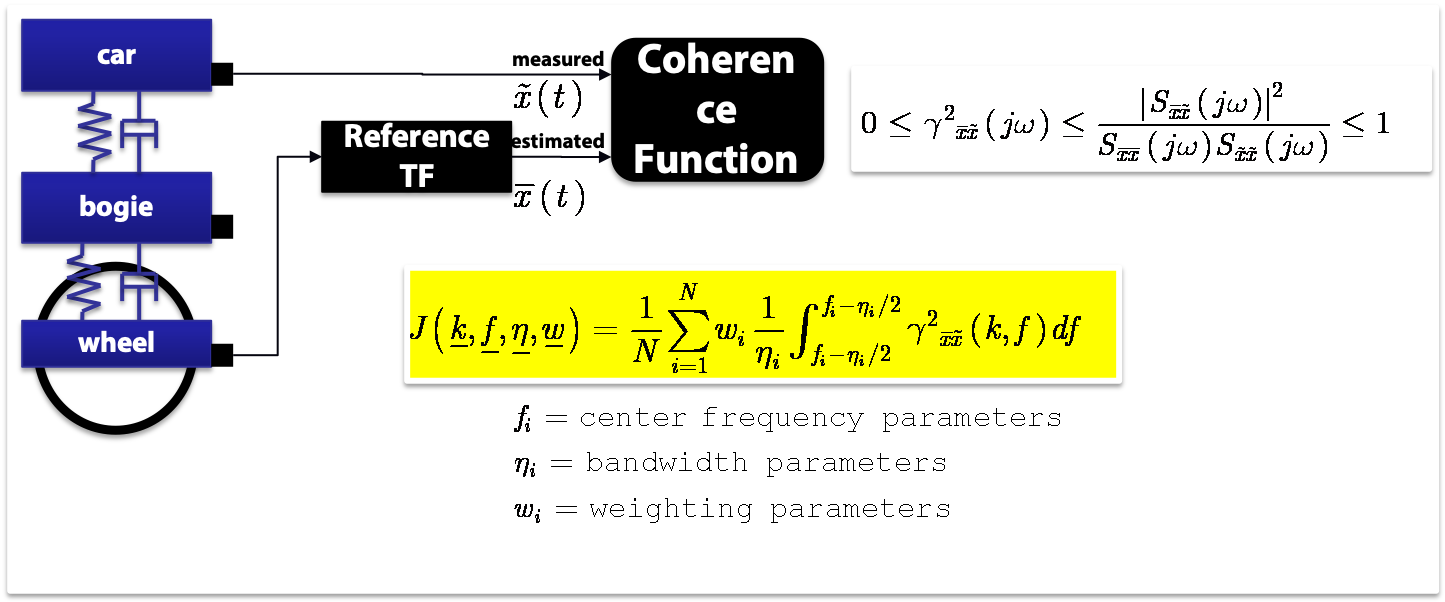
\includegraphics[width=1\textwidth] {images/arex_04.png}
			            \end{fullwidth}
		            \end{figure}
	      \end{itemize}
	\item 개발 스택 및 프레임워크: Mathworks MATLAB / GUI
	\item 참여한 현장:
	      \begin{itemize}
		      \item 코레일 공항철도 (인천-김포)
		      \item 도시철도공사 5호선 (승차감분석, Comfort analysis)
		      \item 코레일 KTX (서울-부산구간)
	      \end{itemize}
\end{itemize}

\cvevent{\printinfo{\faPlusSquare}{초고층 건물의 \href{http://gnss.ngii.go.kr/info/summary}{GNSS} 망조정기법과 외란보정 기법을 이용한 거푸집 연직도 관리}}{Korea Maintenance CO., LTD. 개발참여: 100\%}{Apr. 2009 -- Sep. 2014}{Seoul, Korea}

\begin{itemize}
	\item 소개 : 초고층건물 시공에서 \href{http://gnss.ngii.go.kr/info/summary}{GNSS}를 이용하여 연직도를 관리하고자 하는 신기술 인증 프로젝트
	\item 프로젝트 목표: 거푸집 연직도 시공 누적오차 10mm이내 / 시공 층별오차 4mm 이내의 관리기준을 만족해야 함.
	\item 참여 개발 내용
	      \begin{itemize}
		      \item \href{https://en.wikipedia.org/wiki/Real_Time_Kinematic}{RTK}-\href{https://en.wikipedia.org/wiki/Virtual_Reference_Station}{VRS}\footnote{Virtual Reference Station (VRS) networks use real-time kinematic (RTK) solutions to provide high-accuracy, RTK Global Navigation Satellite Systems.} 시공
		      \item 기준점 네트워크 망조정 : 기준국을 타설하여 3점, 4점 \href{https://en.wikipedia.org/wiki/Procrustes_analysis}{Procrustes}기법을 사용하여 망조정 : OPA\footnote{\href{https://en.wikipedia.org/wiki/Procrustes_analysis}{Ordinary Procrustes Analysis (OPA)}} 방식으로 1초단위의 scale, rotation값을 생성하여 값보정
		      \item 센서퓨전(Sensor fusion) : 가속도계를 설치하여 \href{http://scholar.lib.vt.edu/theses/available/etd-062899-064821/unrestricted/etd.PDF}{Multirate-Kalman Filter (MR-KF)}\footnote{\href{http://scholar.lib.vt.edu/theses/available/etd-062899-064821/unrestricted/etd.PDF}{Multirate-Kalman Filter (MR-KF)}} 사용으로 거푸집의 고속변위예측
		      \item 네트워크 망조정 필터 : 망조정기법에서 scale값과 roation값을 \href{https://ko.wikipedia.org/wiki/\%EC\%B9\%BC\%EB\%A7\%8C_\%ED\%95\%84\%ED\%84\%B0}{칼만 필터(Kalman filter)}로 수정
		      \item 초기 개발단계에서의 개발내용을 전면수정하여 상위의 모든 기술을 적용함
	      \end{itemize}
	\item 적용된 기술
	      \begin{itemize}
		      \item \href{http://gnss.ngii.go.kr/info/summary}{GNSS} (GPS, Glonass) System : \href{http://www.septentrio.com/}{Septentrio} GNSS 적용
		      \item RF 통신 : 각 기준점의 GNSS와 통신
		      \item \href{https://en.wikipedia.org/wiki/Differential_GPS}{Real-time Kinematic Method (DGPS)}
		      \item \href{https://en.wikipedia.org/wiki/Procrustes_analysis}{Ordinary Procrustes Analysis (OPA)}
		      \item \href{http://scholar.lib.vt.edu/theses/available/etd-062899-064821/unrestricted/etd.PDF}{Multirate-Kalman  Filter (MR-KF)}
		      \item \href{http://ieeexplore.ieee.org/xpl/login.jsp?tp=\&arnumber=258116\&url=http\%3A\%2F\%2Fieeexplore.ieee.org\%2Fxpls\%2Fabs_all.jsp\%3Farnumber\%3D258116}{Fourier Linear Combiner (FLC)}
	      \end{itemize}
	\item 개발 스택 및 프레임워크
	      \begin{itemize}
		      \item \href{https://en.wikipedia.org/wiki/National_Instruments}{National Instruments} \href{https://en.wikipedia.org/wiki/LabVIEW}{LabVIEW}
		      \item \href{https://en.wikipedia.org/wiki/MathWorks}{Mathworks} \href{https://en.wikipedia.org/wiki/MATLAB}{MATLAB}
		            \begin{figure}[ht]
			            \begin{fullwidth}
				            \centering
				            \parbox{0.5\textwidth}{
					            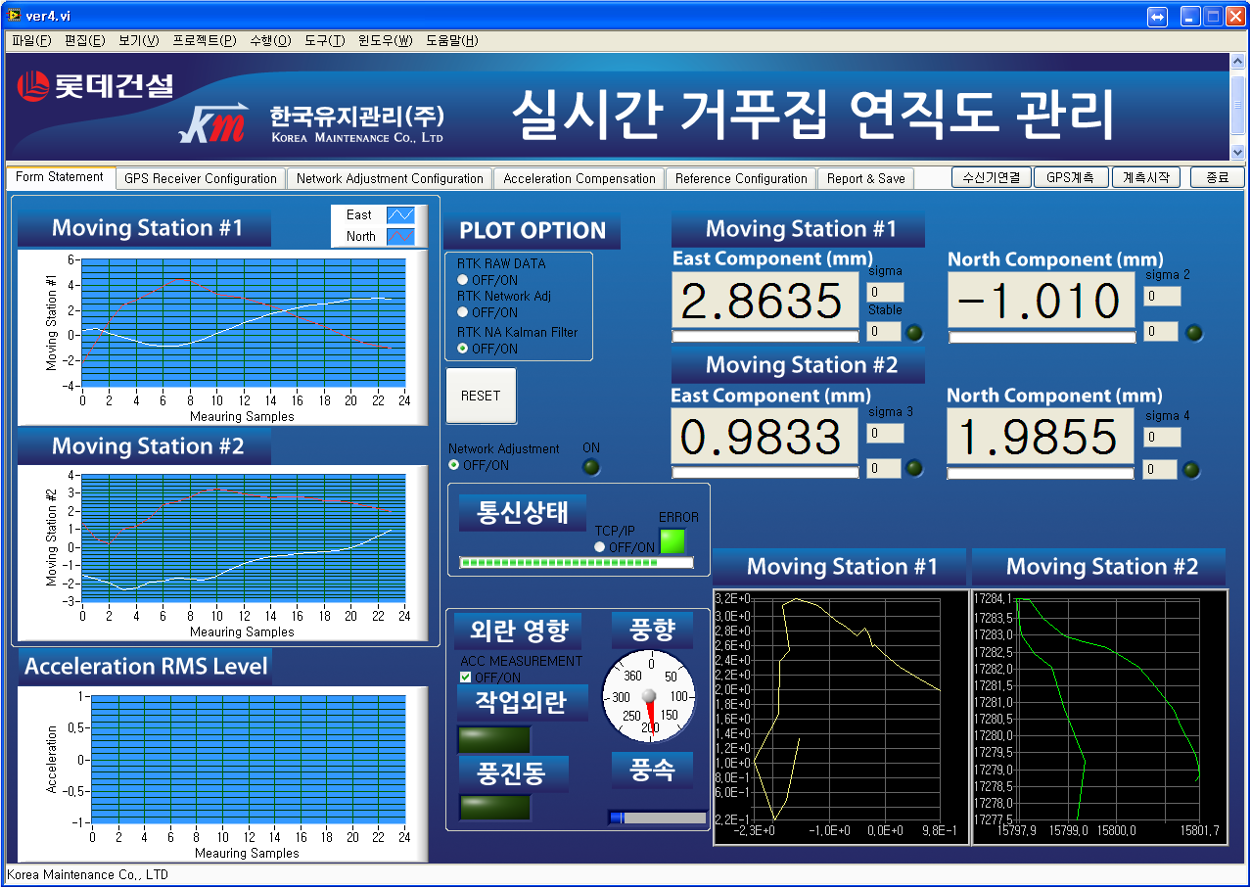
\includegraphics[width=0.5\textwidth] {images/gps_01.png}
					            \caption*{거푸집 연직도관리 SW}
				            }\qquad
				            \parbox{0.5\textwidth}{
					            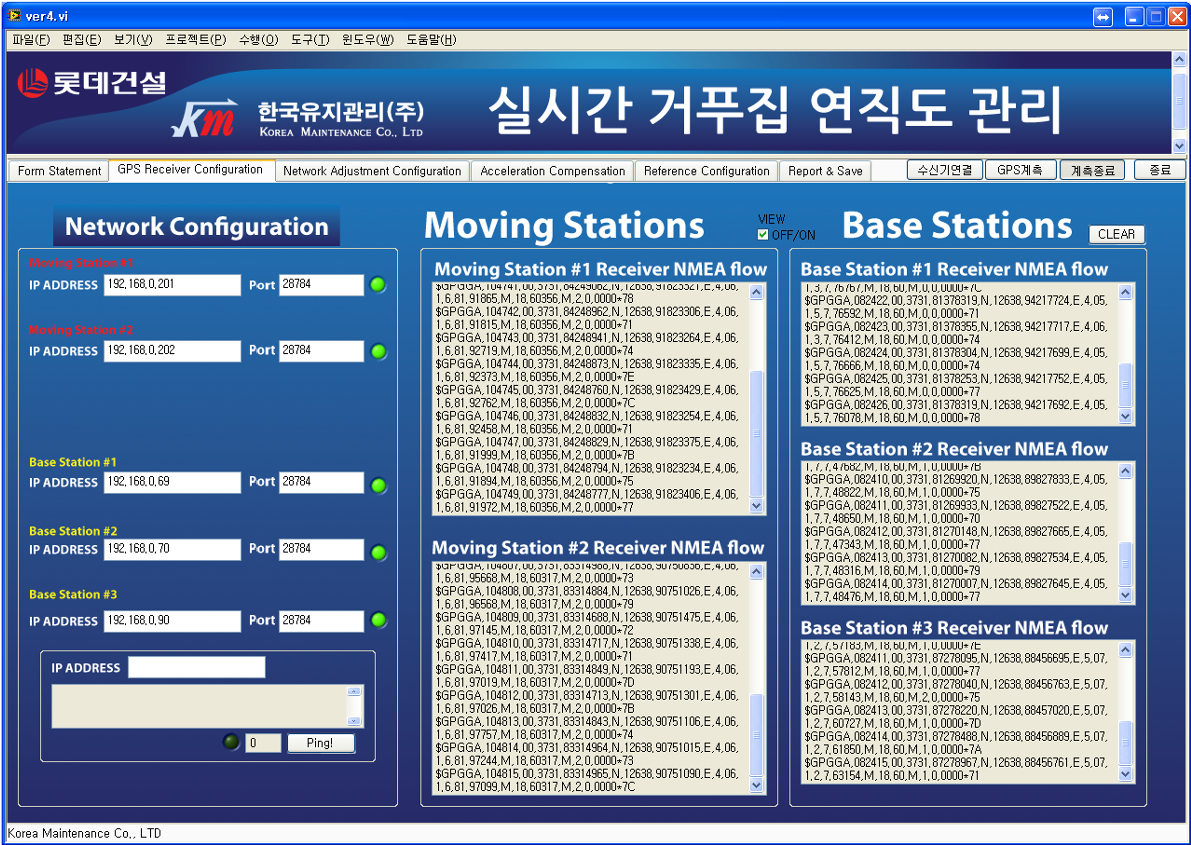
\includegraphics[width=0.5\textwidth] {images/gps_02.png}
					            \caption*{GPS-RTK Streaming}
				            }\qquad
				            \parbox{0.5\textwidth}{
					            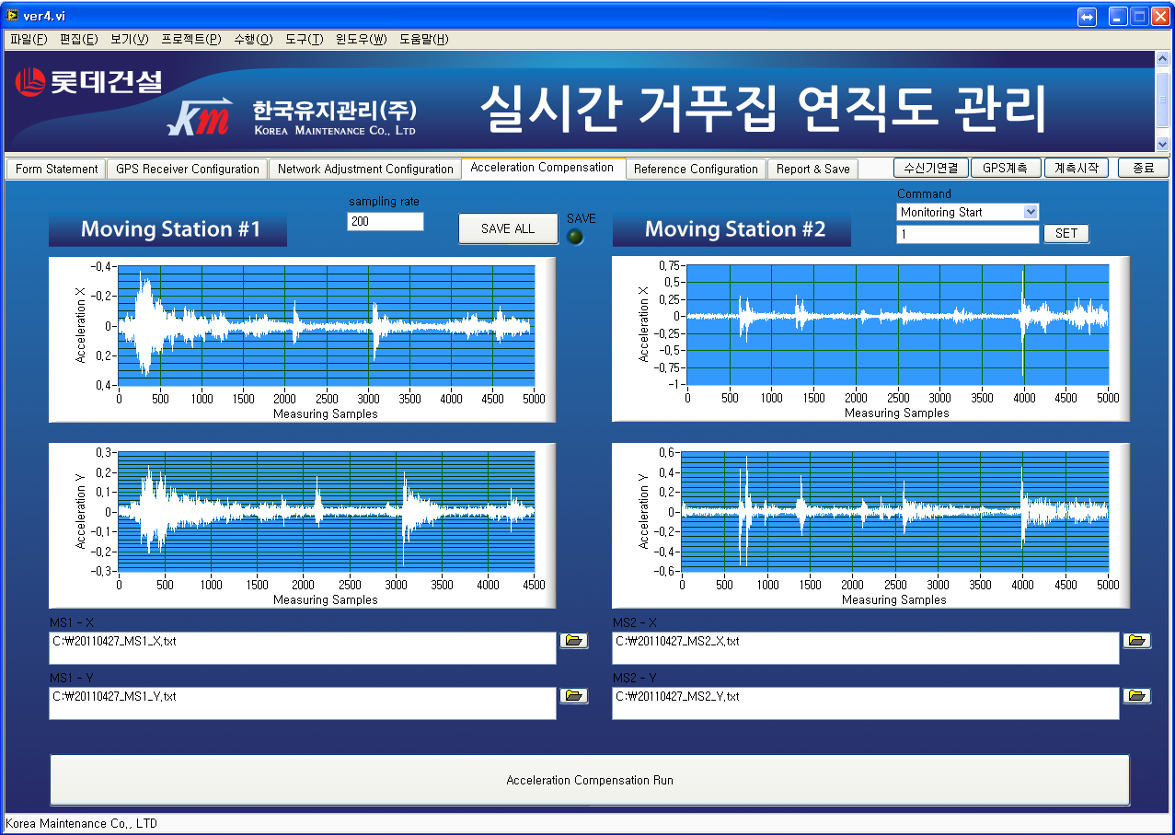
\includegraphics[width=0.5\textwidth] {images/gps_03.png}
					            \caption*{Accelerometer compensation}
				            }
			            \end{fullwidth}
		            \end{figure}
	      \end{itemize}
	\item 참여한 현장
	      \begin{itemize}
		      \item 마포 주상복합 : 후처리 \href{https://en.wikipedia.org/wiki/Differential_GPS}{DGPS} 시스템 적용
		      \item 롯데슈퍼타워 브레이스 위치 측정 : GNSS-RTK만 적용
		      \item 현대제철 당진 코크스 연돌 \href{https://en.wikipedia.org/wiki/Climbing_formwork}{ACS거푸집}\footnote{에이씨에스 자동인양 시스템 (ACS Self Climbing System)} 계측 : 3점망조정 RTK적용
		      \item 부산 연산구 거제동 롯데캐슬피렌체 주상복합 건물 거푸집계측 : 3점망조정, 4점망조정 데이터 (실제 거푸집 시공에 반영)
		      \item 인천 청라지구 롯데케슬 주상복합 건물 거푸집 계측 : 4점망조정 데이터 (신기술 현장실사)
		      \item 인천 청라지구 롯데케슬 주상복합 건물 거푸집 계측 : \href{http://scholar.lib.vt.edu/theses/available/etd-062899-064821/unrestricted/etd.PDF}{MR-KF} 시범적용
	      \end{itemize}
	\item
	      개발결과 : 건설신기술인증
	      \href{http://www.kaia.re.kr/portal/newtec/view.do?searchCnd=1\&searchWrd=\&menuNo=200075\&frApntYear=\&toApntYear=\&pageUnit=10\&frApntNo=\&toApntNo=\&cate1=\&cate2=\&cate3=\&tecCat1=\&tecCat2=\&tecCat3=\&newtecCat1=\&newtecCat2=\&newtecCat3=\&dvlprNm=\%ED\%95\%9C\%EA\%B5\%AD\%EC\%9C\%A0\%EC\%A7\%80\%EA\%B4\%80\%EB\%A6\%AC\&ordDvs=\&pageIndex=1\&apntNo=625\&frMenu=list}{국토해양부고시 제2011 -313호}
\end{itemize}
